\paragraph{}En esta página se puede observar el listado completo de todos los microcontroladores existentes en el catálogo electronico. En la parte derecha de la tabla, tras la especificación de cada microcontrolador, se hallan los siguientes botones:
\begin{itemize}
	\item \textbf{Editar:} Redirige al administrador a la página para editar la especificación y características de dicho microcontrolador.
	\item \textbf{Eliminar:} Elimina el microcontrolador de la base de datos del catálogo electrónico, recargando la página con el nuevo listado actualizado.
\end{itemize}

\begin{figure}[h!]
	\centering
	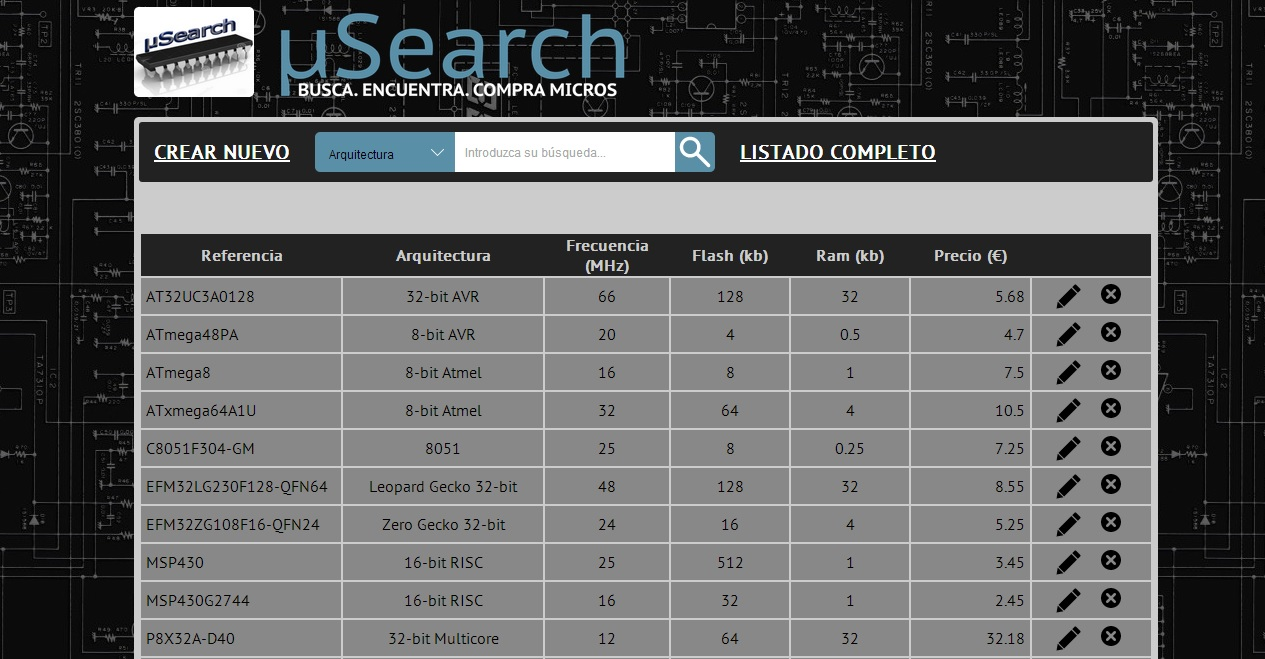
\includegraphics[width=0.85\textwidth]{img/listado_completo_admin}
	\caption{Página de listado completo de micro-controladores.}
	\label{fig:listado_completo_admin}
\end{figure}

Como en todas las demás páginas del sitio web, si se pulsa en cualquiera de los dos logotipos del catálogo $\mu$Search (esquina superior izquierda), el sistema redirigirá al administrador a la página inicial de administración del catálogo.

\paragraph{}Desde esta página, a través de los iconos situados en la cabecera debajo de los logotipos de la web, el administrador puede acceder a:

\begin{itemize}
	
	\item \textbf{Crear Nuevo:} Lleva al administrador a la página de inserción de artículos, donde se puede rellenar los parámetros necesarios para agregar un nuevo microcontrolador al catálogo electrónico.

	\item \textbf{Búsqueda:} Desde esta sección de la cabecera, el administrador puede realizar búsquedas sobre el catálogo de microcontroladores en base a cualquiera de las diferentes características de un microcontrolador (Arquitectura, Frecuencia, Flash, RAM). Simplemente se debe seleccionar una de las características de la lista despegable, introducir el texto a buscar y pulsar sobre el icono de búsqueda.
	El administrador será redirigido a una página donde se le mostrará el resultado de la búsqueda en forma de lista de microcontroladores.
			
	\item \textbf{Listado Completo:} Pulsando sobre este botón/icono se recargará la página actual.
\end{itemize}